\documentclass[12pt]{article}
\usepackage{mathtext}
\usepackage{amsmath}
\usepackage[T2A]{fontenc}
\usepackage[utf8]{inputenc}
\usepackage[russian]{babel}
\usepackage[left=1.5cm, right=1.5cm, top=2cm, bottom=2cm, bindingoffset=0cm]{geometry}
\usepackage{listings}
\usepackage{fancyhdr}
\usepackage{pgfplots}
\pgfplotsset{compat=1.9}



\begin{document}
    \begin{center}
        \textbf{Московский авиационный институт} \\
        \textbf{(Национальный исследовательский университет)}
    \end{center} 
    ~\\
    ~\\
    Институт: «Информационные технологии и прикладная математика» \\
    Кафедра: 805 «Математическая кибернетика»  \\
    Дисциплина: «Численные методы»  
    ~\\
    ~\\
    ~\\
    \begin{center}
        Лабораторная работа №3 \\
        Тема: Решение начально-краевой задачи для дифференциального\\ уравнения 
        эллиптического типа
    \end{center}
    ~\\
    ~\\
    ~\\
    ~\\
    ~\\
    ~\\
    ~\\
    ~\\
    ~\\
    \begin{flushright}
        Студент: ~~~~~~~~~~~~Хахин Максим~~~~~~\\
        Группа: ~~~~~~~~~~~~~~80-403~~~~~~~~~~~~~~~~~\\
        Преподаватель: ~~~~Иванов И. Э.~~~~~~~\\
        Дата: ~~~~~~~~~~~~~~~~~~~~~~~~~~~~~~~~~~~~~~~~~~~\\
        Оценка: ~~~~~~~~~~~~~~~~~~~~~~~~~~~~~~~~~~~~~~~~\\
    \end{flushright}
    ~\\
    ~\\
    ~\\
    ~\\
    ~\\
    ~\\
    ~\\
    ~\\
    ~\\
    ~\\
    ~\\
    ~\\
    ~\\
    ~\\
    ~\\
    \begin{center}
        Москва, 2021
    \end{center}
    \pagestyle{empty}
    \newpage

    \pagestyle{fancy} 
        \fancyhead{}
        \fancyhead[L]{Хахин Максим}
        \fancyhead[R]{М8О-403Б-18} 
    \fancyfoot{} 
    \begin{enumerate}
        \item \textbf{Задание:}\\
        Решить краевую задачу для дифференциального уравнения
        эллиптического типа. Аппроксимацию уравнения произвести с
        использованием центрально-разностной схемы. Для решения дискретного
        аналога применить следующие методы: метод простых итераций (метод
        Либмана), метод Зейделя, метод простых итераций с верхней
        релаксацией. Вычислить погрешность численного решения путем
        сравнения результатов с приведенным в задании аналитическим
        решением. Исследовать зависимость погрешности от сеточных
        параметров.
        \item \textbf{Вариант 9:}\\
        \begin{figure}[h]
            \center{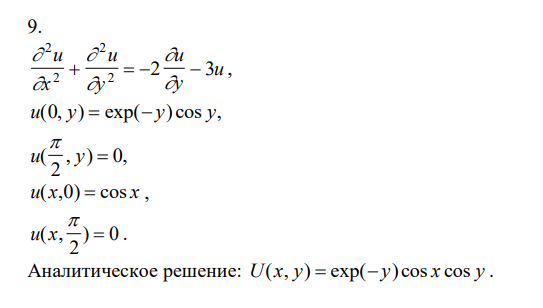
\includegraphics[width=0.5\linewidth]{ 1.png}}
            \label{ris:image}
        \end{figure}\\
        \item \textbf{Теория:}\\
        Рассмотрим уравнение Пуассона, которое является классическим примером 
        эллиптического уравнения:
        $$\frac{\partial^2u}{\partial x^2}+\frac{\partial^2u}{\partial y^2}=f(x,y)$$
        Или уравнение Лапласа при $f(x,y)=0$.
        Первая краевая задача для уравнения Лапласа или Пуассона называется 
        задачей Дирихле:
        $$\begin{cases}
            \frac{\partial^2u}{\partial x^2}+\frac{\partial^2u}{\partial y^2} = f(x,y),~(x,y)\in \Omega;\\
            u(x,y)|_1 = \phi(x,y),~(x,y)\in \Gamma.
        \end{cases}$$
        Если на границе Г задается нормальная производная искомой функции, то 
        соответствующая вторая краевая задача называется задачей Неймана для 
        уравнения Лапласа или Пуассона:
        $$\begin{cases}
            \frac{\partial^2u}{\partial x^2}+\frac{\partial^2u}{\partial y^2} = f(x,y),~(x,y)\in \Omega;\\
            \frac{\partial u(x,y)}{\partial n}\big|_\Gamma = \phi(x,y),~(x,y)\in \Gamma.
        \end{cases}$$
        При этом n – направление внешней к границе Г нормали.\\
        Для решения – строим сетку по x и y. И на ней аппроксимируем задачу во 
        внутренних узлах с помощью отношения конечных разностей по следующей 
        схеме:
        $$\frac{u_{i+1}^j-2u_{i}^j+u_{i-1}^j}{h_x^2}+\frac{u_i^{j+1}-2u_i^j+u_i^{j-1}}{h_y^2}+O(h_x^2+h_y^2) = f(x_i,y_j)$$
        $i = 1...N_x-1,~~j = 1...N_y-1$
        В результате получаем СЛАУ, которую можно решить разными итерационными методами.\\
        1)Метод Либмана:
        $$\frac{u^{k}_{i-1j}-2u^{k+1}_{ij}+u^{k}_{i+1j}}{h_x^2}+\frac{u^{k}_{ij-1}-2u^{k+1}_{ij}+u^{k}_{ij+1}}{h_y^2} = 
        -2\frac{u^{k}_{ij+1}-u^{k}_{ij-1}}{2h_y}-3u_{ij}^k$$
        $$-u^{k+1}_{ij}\left(\frac{2}{h_x^2}+\frac{2}{h_y^2}\right) = -\frac{h_y^2(u^{k}_{i-1j}+u^{k}_{i+1j})-h_x^2(u^{k}_{ij-1}+u^{k}_{ij+1})-
        h_yh_x^2(u^{k}_{ij+1}-u^{k}_{ij-1}) -3h_x^2h_y^2u_{ij}^k}{h_x^2h_y^2}$$
        $$u^{k+1}_{ij} = \frac{(3u_{ij}^kh_x^2 - u^{k}_{i-1j}+u^{k}_{i+1j})h_y^2 + u^{k}_{ij-1}+u^{k}_{ij+1}h_x^2(h_y + 1)}{2h_y^2 + 2h_x^2}$$
        2)Метод Зейделя:
        $$\frac{u^{k+1}_{i-1j}-2u^{k+1}_{ij}+u^{k}_{i+1j}}{h_x^2}+\frac{u^{k+1}_{ij-1}-2u^{k+1}_{ij}+u^{k}_{ij+1}}{h_y^2} = 
        -2\frac{u^{k+1}_{ij+1}-u^{k+1}_{ij-1}}{2h_y}-3u_{ij}^k$$
        $$u^{k+1}_{ij} = \frac{(6u_{ij}^kh_y^2 + (u^{k+1}_{ij+1} - u^{k+1}_{ij-1})h_y + 2u^{k+1}_{ij-1} + 2u^{k}_{ij+1})h_x^2 + 2(u^{k+1}_{i-1j} + 
        u^{k}_{i+1j})h_y^2}{4h_x^2 + 4h_y^2}$$
        
        \item \textbf{Код:}\\
        \begin{lstlisting}[language=C]
        \\Define the initial boundary conditions


double u0y(double y)
{
    return exp(-y)*cos(y);
}
double uly(double y)
{
    return 0;
}
double u0x(double x)
{
    return cos(x);
}
double ulx(double x)
{
    return 0;
}


        \\liebmann_method


void liebmann_method(int N, int K, double Lx, double Ly, double eps, 
double omg, double *args, matrix *grid, double(*f_args[4])(double))
{
    double hx = Lx/(N-1), hy = Ly/(K-1);
    double delta = 1/(2/pow(hx, 2) + 2/pow(hy,2) + args[2]);
    double hhx = 1/pow(hx,2);
    double ahx = args[0]/2/hx;
    double hhy = 1/pow(hy,2);
    double bhy = args[1]/2/hy;
    for(int i=0; i<K; i++)
    {
            *get_element(grid, i, 0) = f_args[2](hx*i);
            *get_element(grid, i, N-1) = f_args[3](hx*i);
    }
    for(int i=0; i<N; i++)
    {
            *get_element(grid, 0, i) = f_args[0](hy*i);
            *get_element(grid, K-1, i) = f_args[1](hy*i);
    }   
    for(int i=1; i<K-1; i++)
        for(int j=1; j<N-1; j++)
        {
            double alpha = (j * hy) / Ly;
            *get_element(grid, i, j) = f_args[2](i * hx)*(1 - alpha) + 
            f_args[3](i * hx) * alpha;
        }
    int n = 0;
    double err = eps*100;
    double *U2;
    do
    {
        n++;
        U2=malloc(N*K*sizeof(double));
        for(int i=0; i<grid->rows; i++)
            for(int j=0; j<grid->columns; j++)
                U2[i*(grid->columns)+ j] = *get_element(grid, i, j);
        
        for(int i=1; i<K-1; i++)
            for(int j=1; j<N-1; j++)
                *get_element(grid, i, j) = delta * ((hhx + ahx) * 
                U2[(i - 1)*N+ j] + (hhx - ahx) * U2[(i + 1)*N+ j] + 
                (hhy + bhy) * U2[i*N+ (j-1)] + (hhy - bhy) * U2[i*N+ (j+1)]);
        err = eror(grid, U2);
        free(U2);
    } while((err > eps) && (n<10000));
    printf("%d", n);
}

            \\seidel_method


void seidel_method(int N, int K, double Lx, double Ly, double eps, 
double omg, double *args, matrix *grid, double(*f_args[4])(double))
{
    double hx = Lx/(N-1), hy = Ly/(K-1);
    double delta = 1/(2/pow(hx, 2) + 2/pow(hy,2) + args[2]);
    double hhx = 1/pow(hx,2);
    double ahx = args[0]/2/hx;
    double hhy = 1/pow(hy,2);
    double bhy = args[1]/2/hy;
    for(int i=0; i<K; i++)
    {
            *get_element(grid, i, 0) = f_args[2](hx*i);
            *get_element(grid, i, N-1) = f_args[3](hx*i);
    }
    for(int i=0; i<N; i++)
    {
            *get_element(grid, 0, i) = f_args[0](hy*i);
            *get_element(grid, K-1, i) = f_args[1](hy*i);
    }   
    for(int i=1; i<K-1; i++)
        for(int j=1; j<N-1; j++)
        {
            double alpha = (j * hy) / Ly;
            *get_element(grid, i, j) = f_args[2](i * hx)*(1 - alpha) + 
            f_args[3](i * hx) * alpha;
        }
    int n = 0;
    double err = eps*100;
    double *U2;
    do
    {
        n++;
        U2=malloc(N*K*sizeof(double));
        for(int i=0; i<grid->rows; i++)
            for(int j=0; j<grid->columns; j++)
                U2[i*(grid->columns)+ j] = *get_element(grid, i, j);
        
        for(int i=1; i<K-1; i++)
            for(int j=1; j<N-1; j++)
                *get_element(grid, i, j) = delta * ((hhx + ahx) * 
                (*get_element(grid, i-1, j)) + (hhx - ahx) * 
                (*get_element(grid, i+1, j)) + (hhy + bhy) * 
                (*get_element(grid, i, j-1)) + (hhy - bhy) * 
                (*get_element(grid, i, j+1)));
        err = eror(grid, U2);
        free(U2);
    } while((err > eps) && (n<10000));
    printf("%d", n);
}


            \\relax_method


void relax_method(int N, int K, double Lx, double Ly, double eps,
double omg, double *args, matrix *grid, double(*f_args[4])(double))
{
    double hx = Lx/(N-1), hy = Ly/(K-1);
    double delta = 1/(2/pow(hx, 2) + 2/pow(hy,2) + args[2]);
    double hhx = 1/pow(hx,2);
    double ahx = args[0]/2/hx;
    double hhy = 1/pow(hy,2);
    double bhy = args[1]/2/hy;
    for(int i=0; i<K; i++)
    {
            *get_element(grid, i, 0) = f_args[2](hx*i);
            *get_element(grid, i, N-1) = f_args[3](hx*i);
    }
    for(int i=0; i<N; i++)
    {
            *get_element(grid, 0, i) = f_args[0](hy*i);
            *get_element(grid, K-1, i) = f_args[1](hy*i);
    }   
    for(int i=1; i<K-1; i++)
        for(int j=1; j<N-1; j++)
        {
            double alpha = (j * hy) / Ly;
            *get_element(grid, i, j) = f_args[2](i * hx)*(1 - alpha) +
             f_args[3](i * hx) * alpha;
        }
    int n = 0;
    double err = eps*100;
    double *U2;
    do
    {
        n++;
        U2=malloc(N*K*sizeof(double));
        for(int i=0; i<grid->rows; i++)
            for(int j=0; j<grid->columns; j++)
                U2[i*(grid->columns)+ j] = *get_element(grid, i, j);
        
        for(int i=1; i<K-1; i++)
            for(int j=1; j<N-1; j++)
                *get_element(grid, i, j) = (*get_element(grid, i, j)) +
                 omg * (delta * ((hhx + ahx) * (*get_element(grid, i-1, j))+
                (hhx - ahx) * U2[(i + 1)*N+ j] + (hhy + bhy) *
                (*get_element(grid, i, j-1)) +(hhy - bhy) *
                U2[i*N+ (j+1)]) - (*get_element(grid, i, j)));
        err = eror(grid, U2);
        free(U2);
    } while((err > eps) && (n<10000));
    printf("%d", n);
}
\end{lstlisting}
        \item \textbf{Результат:}\\
        Метод Либмана:
        \begin{figure}[h]
            \center{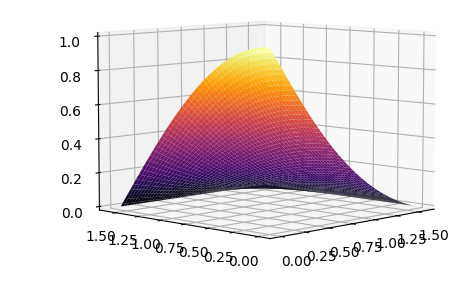
\includegraphics[width=0.5\linewidth]{ 2.png}}
            \label{ris:image}
        \end{figure}\\
        \newpage
        Покажем ошибку в зависимости от длины шага по пространству
        \begin{figure}[h]
            \center{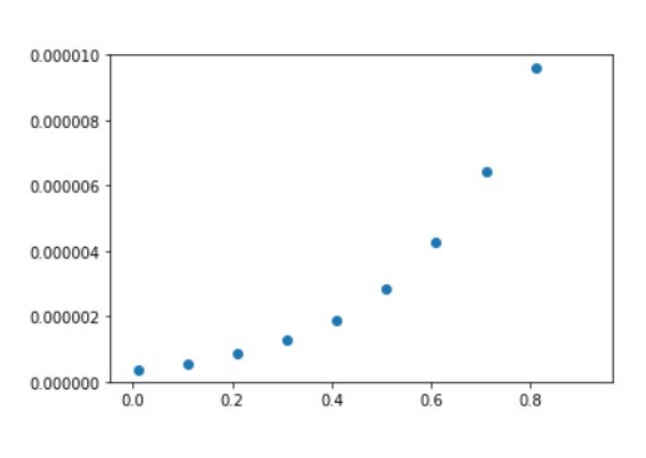
\includegraphics[width=0.5\linewidth]{ 3.png}}
            \label{ris:image}
        \end{figure}\\
        Метод Зейделя:
        \begin{figure}[h]
            \center{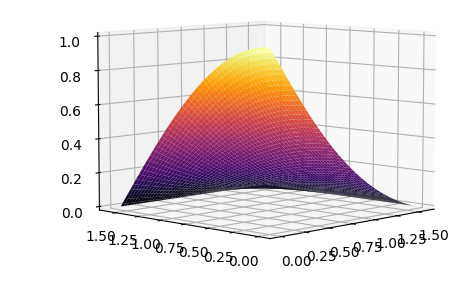
\includegraphics[width=0.5\linewidth]{ 2.png}}
            \label{ris:image}
        \end{figure}\\
        Покажем ошибку в зависимости от длины шага по пространству
        \begin{figure}[h]
            \center{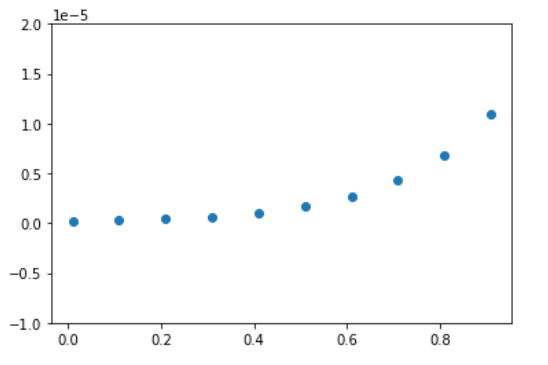
\includegraphics[width=0.4\linewidth]{ 4.png}}
            \label{ris:image}
        
        \end{figure}\\
        \newpage
                Метод Релаксации:
        \begin{figure}[h]
            \center{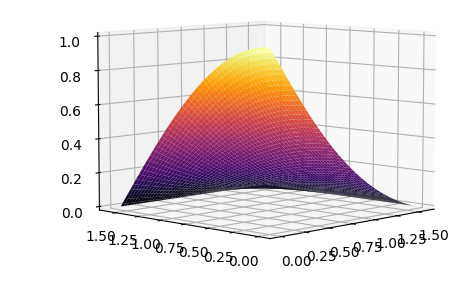
\includegraphics[width=0.5\linewidth]{ 2.png}}
            \label{ris:image}
        \end{figure}\\
        Покажем ошибку в зависимости от длины шага по пространству

        \begin{figure}[h]
            \center{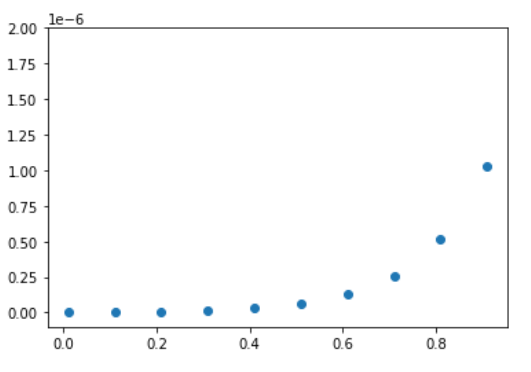
\includegraphics[width=0.4\linewidth]{ 5.png}}
            \label{ris:image}
        \end{figure}\\

        \newpage


        \item \textbf{Вывод:}\\
        В лабораторной работе №3 изучил методы Либмана, Зейделя и Релаксации, построил 
        график зависимости ошибки от размера шага по пространству и сравнил 
        количество итераций для выполнения алгоритма в заданой точности: 
        \\1)При 100х100 сетка 0.00001 эпсилон;
        \\Простые 5000;
        \\Зейдель 3400;
        \\Релаксация 1600;
        \\2)При 50х50 сетка 0.00001 эпсилон;
        \\Простые 2157;
        \\Зейдель 1606;
        \\Релаксация 554;
        \\3)При 25х25 сетка 0.00001 эпсилон;
        \\Простые 739;
        \\Зейдель 425;
        \\Релаксация 169;

    \end{enumerate}
\end{document}